% =======================================
% 参考文献
% =======================================

\bibliography{src/E-Reference}

% 引用所有 E-Reference.bib 里面的全部参考文献,不论在论文中是否被引用
\nocite{*}


\appendix
\section{主要使用的软件}

\begin{enumerate}
    \item 文字编辑方案:Visual Studio Code + \LaTeX + Git + Zotero
    \item 程序模拟:PyCharm + Python
    \item 绘图软件:XMind + PyCharm + Python + GeoGebra
\end{enumerate}

\section{程序代码}

\begin{lstlisting}[caption={类的定义语句}]
    #include<iostream>
    using namespace std;

    int main(){
        cout << "Hello, 数学建模" << endl;
        return 0;
    }
\end{lstlisting}

\section{GeoGebra绘制链接}

\begin{enumerate}
    \item \href{https://www.geogebra.org/m/fza22fcy}{\textcolor{blue}{问题一重述图}}
    \item \href{https://www.geogebra.org/m/hpkkarys}{\textcolor{blue}{问题一求解图}}
    \item \href{https://www.geogebra.org/m/f6kfjvru}{\textcolor{blue}{问题二求解图}}
    \item \href{https://www.geogebra.org/m/n8saurfn}{\textcolor{blue}{测坡角与测线方向角的函数图像}}
    \item \href{https://www.geogebra.org/m/xcvstdzg}{\textcolor{blue}{理想情况下的覆盖区域几何图}}
    \item \href{https://www.geogebra.org/m/absuxwpk}{\textcolor{blue}{一般情况下的覆盖区域几何图}}
    \item \href{https://www.geogebra.org/m/jzwhwcqr}{\textcolor{blue}{一般情况下通式计算几何图}}
\end{enumerate}

\section{两张图片并排放置案例}

\begin{figure}[htbp]
    \centering
    \begin{subfigure}[b]{0.45\textwidth}
      \centering
      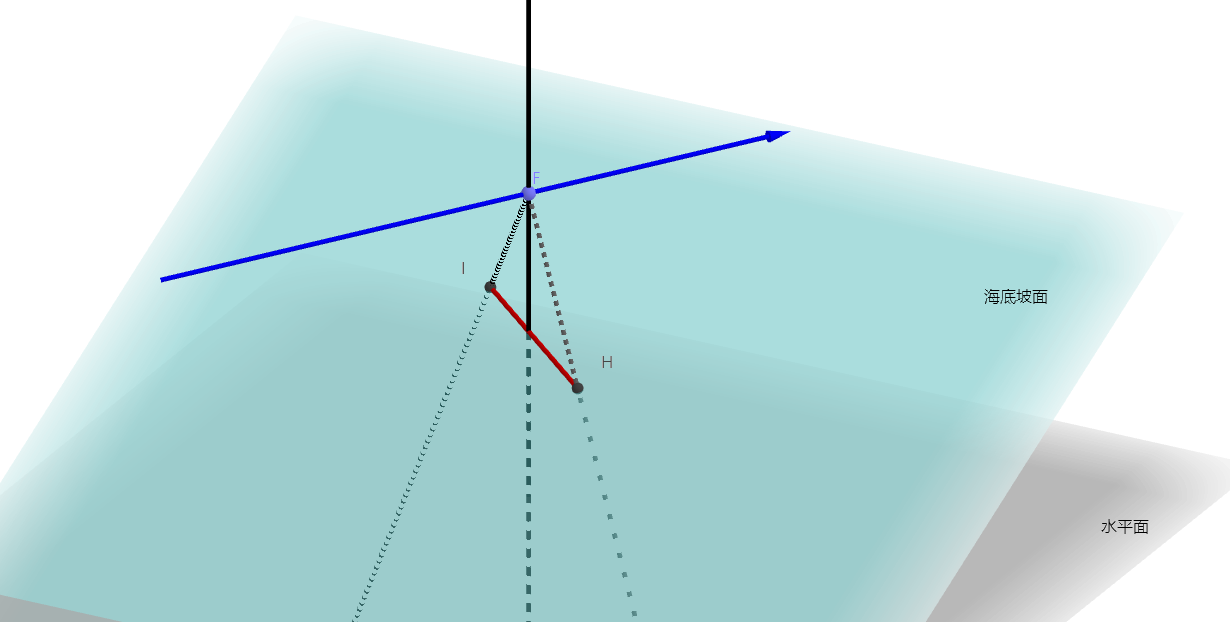
\includegraphics[width=\textwidth]{res/img/测坡面示意图.png}
      \caption{图像1}
      \label{fig:image1}
    \end{subfigure}
    \hfill
    \begin{subfigure}[b]{0.45\textwidth}
      \centering
      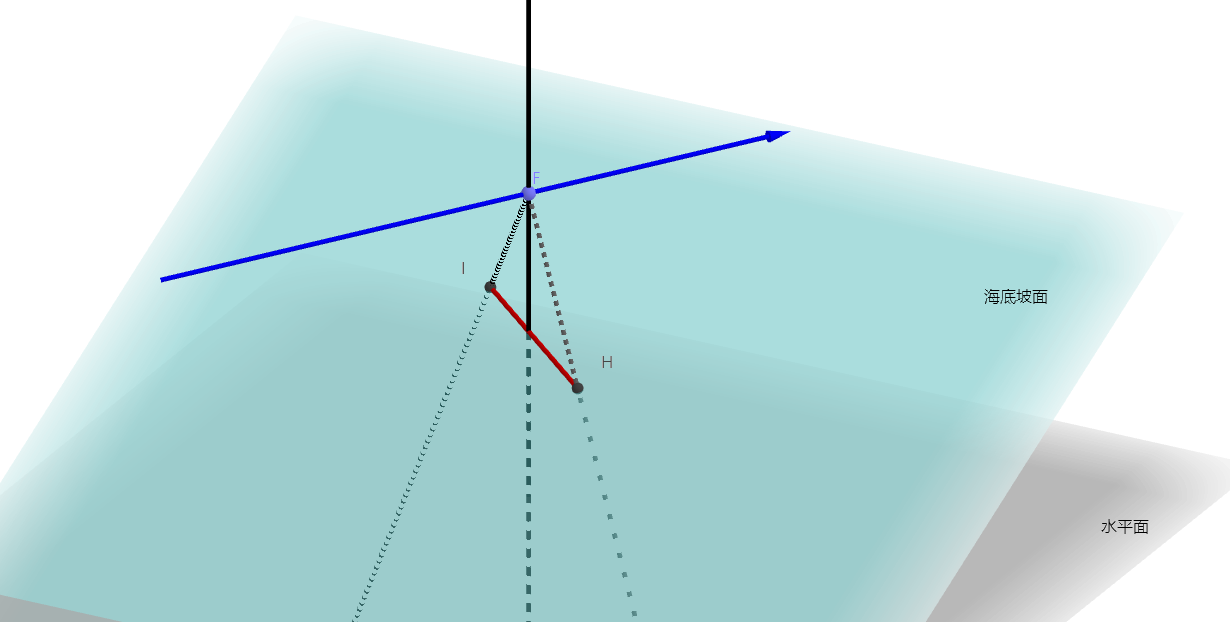
\includegraphics[width=\textwidth]{res/img/测坡面示意图.png}
      \caption{图像2}
      \label{fig:image2}
    \end{subfigure}
    \caption{两张图片的子标题}
    \label{fig:two_images}
  \end{figure}